\addchap{Modulübersicht}

Ein (M) kennzeichnet ein Modul nur für Medieninformatiker, ein (I) jeweils Module für Informatiker und ein (D) für Diplominformatiker.

\minisec{{\Large\ \\ 1. Semester\\\ }}

\textbf{\menu[,]{I, M, D, Einführung in die Mathematik für Informatiker\,}}\\
Du kennst dich mit Matrizen aus?
Dann weißt du auch was mit den Begriffen Determinante, Diagonalisierbarkeit, Skalarprodukt und der Lösung eines homogenen linearen Gleichungssystems anzufangen - wenn nicht, dann lernst du es hier von der Pike an.
Außerdem wird in der Diskreten Mathematik das Mal und Plus quasi neu definiert und du lernst ein wenig anders zu denken.

\textbf{\menu[,]{I, M, D, Algorithmen und Datenstrukturen\,}} \\
Was kommt zuerst?
5 oder 3?
Solche Fragen werden dich in Algorithmen und Datenstrukturen beschäftigen während du Quicksort, Heapsort und Konsorten lernt.
% Der Wortwitz gefällt mir...
Weiter wirst du dich als Gärtner versuchen indem du AVL- und andere Bäume wachsen lasst.
Dabei wirst du Bekanntschaft mit der Programmiersprache C machen.

\textbf{\menu[,]{I, M, D, Einführungspraktikum\,}} \\
Du hast schon immer gerne mit Lego gespielt?
Dann wird dir dieses Praktikum, welches in der vorlesungsfreien Zeit stattfindet, gefallen.
Du darfst dich im Team daran machen einen selbst konstruierten Roboter in C beizubringen, wie er sich in einem Labyrinth alleine zurechtfindet.
Dabei, und im anschließenden Wettbewerb, kommt der Spaß nicht zu knapp.
Für Diplomstudenten gibt es zusätzlich ein einwöchiges Einzelprojekt, bei dem man zeigen kann, was man in C oder wahlweise C++ drauf hat. Alternativ kann das Strategiespielepraktikum auch auf das Sommersemester verschoben werden.
Im letzten Jahr war eine KI für bekannte Brettspiele gefragt.

\textbf{\menu[,]{I, M, Einführung in die Medieninformatik\,}} \\
Anfangs erfolgt eine Darstellung des menschlichen Wahrnehmungssystems, Aspekte der Wahrnehmungspsychologie und der Softwareergonomie.
Dann werden Eigenschaften der Information und Datenformate anhand der Medien Text, Bild, Audio und Video dargestellt.
Im Bereich Text und Bild werden die entsprechenden Dokumentenformate des Internet (HTML und SVG) besprochen.
Ein weiterer Teil der Lehrveranstaltung gibt einen Überblick zur Dokumentenverarbeitung mittels XML-Techniken.
In Übungen und in Form eines Projektes in einer kleinen Gruppe über das Semester hinweg hast du die Möglichkeit, das Erlente direkt in die Praxis umzusetzen.

\textbf{\menu[,]{D, Technische Grundlagen und Hardwarepraktikum\,}} \\
$\rightarrow$ 3. Semester

\textbf{\menu[,]{D, Rechnerarchitektur\,}} \\
$\rightarrow$ 3. Semester


\minisec{{\Large\ \\ 2. Semester\\\ }}

\textbf{\menu[,]{I, M, D, Mathematische Methoden für Informatiker\,}} \\
Nachdem der Abistoff viel tiefer als vorher sitzt, geht es in den nächsten zwei Semestern in neue Bereiche der Mathematik.
Anfangs werden die verschiedenen Typen algebraischer Strukturen (das sind Mengen von beliebigen Symbolen und darauf erklärte Rechenoperationen) untersucht.
Es folgen Vektoren, Matrizen und mathematische Körper.
Dann kommt ein Sprung vom Diskreten zum Kontinuierlichen.
So langweilig wie in der Schule ist Analysis nämlich gar nicht, die gibt es auch in der Ausführung mit mehreren Veränderlichen.
Das Ganze gipfelt in der Einführung von Differentialgleichungen.
Gegen Schluss wendet man sich erneut den Polynomen zu.
Dabei werden zunächst effiziente Näherungsverfahren behandelt.
Später folgt dann ein kurzer Ausflug in die Stochastik.

\textbf{\menu[,]{I, M, D, Programmierung\,}} \\
Dass Programmiersprachen nicht auf Bäumen wachsen, wusstest du wahrscheinlich schon, doch dass sie strengen mathematischen Regeln folgen, lernst du hier.
Am Beispiel eines Teils der Programmiersprache C wird zunächst die Syntax mit Hilfe von Grammatiken definiert.
Kurz darauf kommst du in den Kontakt mit der funktionalen Programmiersprache Haskell.
Durch viele hübsche, rekursiv verschachtelte Abbildungen wird dann die Semantik festgelegt, d.h. die Wirkung, die so ein Programm auf einer (abstrakten) Rechenmaschine hat.
Hier wird auch vermittelt, wie man die Korrektheit eines Programmstückes \glqq wasserdicht\grqq, d.h. formal logisch beweisen kann.

\textbf{\menu[,]{I, M, D, Informations- und Kodierungstheorie\,}} \\
Was Informationen eigentlich sind, was sie ausmacht, wird dich hier beschäftigen.
In dieser Lehrveranstaltung wirst du einen Einstieg in ein sehr interessantes und komplexes Fachgebiet erhalten.
Im Mittelpunkt steht am Anfang wie man Informationen darstellen und speichern kann.
Etwas später wird erklärt, warum und wie die Informationen mittels Kodierung geschützt werden, damit sie bei dir sicher ankommen, wenn sie unterwegs Störungen und Manipulationen ausgesetzt sind.
Dabei wird dir dein in der Mathematik erworbenes Wissen von Nutzen sein.

\textbf{\menu[,]{I, M, D, Softwaretechnologie\,}} \\
Software zu entwickeln ist eine Kunst, das wirst du spätestens nach diesem Modul erkennen.
Um diese Kunstfertigkeit an den Tag legen zu können bedarf es einiger Handwerkszeuge, welche du hier mit auf den Weg bekommst.
So werden dir moderne Konzepte am Beispiel von Java und Entwurfsverfahren zusammen mit professioneller Dokumentation näher gebracht.
Damit wird dann der Grundstein für das Projekt im dritten Semester gelegt, bei dem man sich Lorbeeren im Projektmanagement und als Entwickler verdienen kann.

\textbf{\menu[,]{I, M, Einführung in die Computergraphik\,}} \\
Es geht um den Aufbau von Grafiksystemen, Farbräumen, Rastergraphiken und deren Anwendungen.
Bestehende Probleme, wie Aliasing und Artefakte sind mit von der Partie, sowie ihre algorithmischen Lösungen.
Als Programmiersprache für die Übungsaufgaben wird C++ genutzt.

\textbf{\menu[,]{D, Technische Grundlagen und Hardwarepraktikum\,}} \\
Fortsetzung aus dem 1. Semester.

\textbf{\menu[,]{D, Rechnerarchitektur\,}} \\
Fortsetzung aus dem 1. Semester.


\minisec{{\Large\ \\ 3. Semester\\\ }}

\textbf{\menu[,]{I, M, D, Mathematische Methoden für Informatiker\,}} \\
Fortsetzung aus dem 2. Semester.

\textbf{\menu[,]{I, M, D, Formale Systeme\,}} \\
Wahr?
Und oder falsch?
Was falsch ist wird, wenn es falsch falsch ist, wahr?
Logisch!
Neben der Aussagenlogik vermittelt das Modul die Grundlagen formaler Sprachen.
Es folgen Gedanken zu maschinellen Berechenbarkeit und zur Automatentheorie.
Turing lässt grüßen.

\textbf{\menu[,]{I, M, D, Softwaretechnologie-Projekt\,}} \\
Das Projekt nimmt den größten Teil des dritten Semesters ein.
Hier muss man sein Wissen aus der Lehrveranstaltung \glqq Softwaretechnologie\grqq\ in die Tat umsetzen.
In einem fünfköpfigen Team hast du die Aufgabe, eine Anwendung für einen realen Kunden oder den Lehrstuhl von vorn bis hinten fertig zu stellen.
Dabei muss man häufig Rücksprache mit den Kunden halten.
Abgeschlossen wird das Modul mit einer Präsentation des fertigen Produkts vor dem Kunden und den Verantwortlichen des Moduls.
Am Ende hast du dann einen Eindruck, wie die Arbeit eines Informatikers aussehen kann.

\textbf{\menu[,]{I, M, Rechnerarchitektur\,}} \\
Hier geht es um die Grundbausteine eines Computers:
Speicher, Bussysteme, Rechen- und Steuerwerk.
Außerdem erhält man eine Einführung in Assembler, das Pipelining-Prinzip und damit auftretende Probleme.
Schließlich wird noch diskutiert, mit welchen Methoden man heutige Rechnerarchitekturen beschleunigen kann und parallele Architekturen nutzen kann.

\textbf{\menu[,]{I, Technische Grundlagen und Hardwarepraktikum\,}} \\
Wer schon immer mal wissen wollte, was die Elektronen im häuslichen Rechner eigentlich so alles durchmachen müssen, bekommt das genau vermittelt.
Anfangs werden Transistor-, Dioden- und Operationsverstärkerschaltungen betrachtet.
Darauf aufbauend geht es über Verknüpfungsglieder und komplexe Schaltungen.

\textbf{\menu[,]{M, Grundlagen der Gestaltung\,}} \\
Die Vorlesung beginnt mit Begriffsdefinitionen sowie allgemeinen Gestaltungsprinzipien und erläutert diese.
Dabei beschränkt sich die Veranstaltung bewusst auf zweidimensionale Bereiche.
Formkategorien, Kontrastbildung und Farblehre bilden die Schwerpunkte.
Die begleitenden Übungen sollen einen Einblick in die Materie vermitteln und die Sensibilität der Studierenden durch handwerkliches Arbeiten wecken.

\textbf{\menu[,]{D, Grundlagen des Nebenfachs\,}} \\
Je nachdem, was du dir als Nebenfach wählst, beschäftigst du dich hier mit Themen die nur im entfernten Sinne mit Informatik zusammenhängen.
Über den Tellerrand schauen und andere Welten kennenlernen ist das Motto.

\textbf{\menu[,]{D, Betriebssysteme und Sicherheit\,}} \\
$\rightarrow$ 5. Semester


\newpage

\minisec{{\Large\ \\ 4. Semester\\\ }}

\textbf{\menu[,]{I, D, Theoretische Informatik und Logik\,}} \\
Die Fortsetzung der Formalen Systeme.
Es folgen weitere Betrachtungen zur Korrektheit und Terminierung von Algorithmen und der notwendige Aufwand in Form von Zeit und Platzbedarf.
Ein Abstecher in die Prädikatenlogik und Logikprogrammierung rundet das Modul ab.

\textbf{\menu[,]{I, M, Rechnerarchitektur\,}} \\
Fortsetzung aus dem 3. Semester.

\textbf{\menu[,]{I, M, D, Datenbanken und Rechnernetze\,}} \\
Dies Modul besteht aus zwei verschiedenen Lehrveranstaltungen.
In Datenbanken lernt man zuerst Methoden zur effizienten Datenspeicherung kennen.
Danach wird die Fähigkeit vermittelt, selbst komplexe relationale Datenbanken zu konzipieren und zu erstellen.
In Rechnernetze wird angefangen mit dem Funktionsprinzip von Modem und Netzwerkkarte und man erhält einen kurzen Überblick über moderne Kommunikations- und Vermittlungsprotokolle.
Auch der Sektor Mobilkommunikation und die dabei auftretenden Schwierigkeiten werden kurz beleuchtet.

\textbf{\menu[,]{I, Technische Grundlagen und Hardwarepraktikum\,}} \\
Fortsetzung aus dem 3. Semester.

\textbf{\menu[,]{M, Einführung in die Mediengestaltung\,}} \\
Die Vorlesung vermittelt die Grundzüge des multimedialen Gestaltens unter Gesichtspunkten der Entwicklung der einzelnen Richtungen (Film, Internet) mit Bezug auf die gestalterischen Änderungen in den vergangenen Jahrhunderten (Buch).
Außerdem wird in die Metaphernbildung eingeführt und es werden Schwerpunkte in Richtung des Interfacedesign gesetzt.

\textbf{\menu[,]{M, Medien und Medienströme\,}} \\
Hier wird Wissen zu Medien, deren Kompression und Bearbeitung vermittelt.
Die Anwendung verschiedener Werkzeuge zur Erzeugung von Medien und deren Charakteristika sind ebenfalls Gegenstand dieser Lehrveranstaltung.
So wirst du dich in Form von Übungsaufgaben mit den Grundlagen der Bild-, Audio- und Videobearbeitung auseinandersetzen.

\textbf{\menu[,]{M, Medienpsychologie und -didaktik\,}} \\
Mediendidaktik ist die \glqq Kunst des Lehrens\grqq.
Hier werden die Fragen beantwortet:
Was ist Bildung?
Wie verläuft sie?
Wie lässt sie sich vervollkommnen?
Man erfährt etwas über die Entwicklung von Lehrmethoden.
Im parallel stattfindenden Praktikum wird das Gelernte gleich praktisch bei der Entwicklung eines Lernspiels angewandt.

\textbf{\menu[,]{M, Komplexpraktikum\,}} \\
Das große Highlight für Medieninformatiker im Bachelor.
In kleineren Gruppen soll ein mobiles Spiel, eine Internet-Seite oder Multimediales realisiert werden.
Abgesehen von der Aufgabenstellung sind der Fantasie quasi keine Grenzen gesetzt.
Es geht um harte Arbeit, Teamgeist und das Ernten der wohlverdienten Lorbeeren.

\textbf{\menu[,]{D, Forschungslinie\,}} \\
Hier bekommst du einen Überblick über aktuelle Forschungsthemen und bekommst vermittelt, wie man forschungsorientiert arbeitet.
Dieses Modul hilft, später die richtige Vertiefung zu wählen.

\textbf{\menu[,]{D, Grundlagen des Nebenfachs\,}} \\
Fortsetzung aus dem 3. Semester.

\textbf{\menu[,]{D, Allg. Basisqualifikationen\,}} \\
Englisch ist die einzig relevante Sprache in der Informatik.
Hier wird dir vermittelt, wie man sich fachlich auf Englisch ausdrückt.
Abgerundet wird das Modul durch eine Schulung deiner Vortragsfähigkeiten.


\minisec{{\Large\ \\ 5. Semester\\\ }}

\textbf{\menu[,]{I, M, Betriebssysteme und Sicherheit\,}} \\
Diese Lehrveranstaltung nimmt die dienstbaren Geister, die zwischen der Hardware und den bunten Anwendungen werkeln, unter die Lupe.
Warum kann man mit einem Rechner gleichzeitig einen Text schreiben, Code kompilieren, ein Bild bearbeiten und Musik hören?
Wie werden meine Daten in Rechnersystemen geschützt?
Wieso stehen die hier auf dieses Unix?

\textbf{\menu[,]{I, D, Systemorientierte Informatik/Hardware Software Codesign\,}} \\
Dieses Fachgebiet ist die Schnittstelle zwischen Rechnern und der industriellen Praxis, die von der Steuerung von Heizventilen bis zu Kraftwerken reicht.
Zunächst wird abstrahiert, was allen praktisch vorkommenden Systemen gemein ist, und es werden Modelle wie \glqq System\grqq, \glqq Signal\grqq\ und \glqq Regelkreis\grqq\ erschaffen, mit denen sich dann rechnerisch umgehen lässt.
Hier wird man fit gemacht für die Analyse und Voraussage von Übertragungsverhalten und Reaktionen, die ein solches System bei einem bestimmten Input zeigen wird.
Daneben kommen auch Aspekte aus der Audio- und Videotechnik wie Digitalisierung und Filteralgorithmen nicht zu kurz.

\textbf{\menu[,]{I, D, Intelligente Systeme\,}} \\
In dieser Lehrveranstaltung geht es um künstliche Intelligenz.
Hier erlernt man Problemlösung, Wissensrepräsentation, Planung, Wahrnehmung und Sprachverstehen mit Hilfe spezieller Algorithmen und Agenten.

\textbf{\menu[,]{M, Web- und Multimedia Engineering\,}} \\
Wie kann man das Web mit heutiger Technik multimedial und interaktiv gestalten?
Wie nutze ich professionelle Entwicklungswerkzeuge und geeignete Sprachen, wie z.B. Java, um meine Vorstellung in das Ergebnis zu projizieren?
% professionelle Entwicklungswerkzeuge und geeignete Sprachen (im Bezug auf Webentwicklung) -> Java... Alles klar m(
Dieses Modul hilft geeignete Methoden zu erlernen und Erfahrung bei der Anwendung zu sammeln.

\textbf{\menu[,]{M, Komplexpraktikum\,}} \\
Fortsetzung aus dem 4. Semester.

\textbf{\menu[,]{I, M, D, Vertiefung\,}} \\
Hier kannst du aus einem Angebotskatalog geeignete Veranstaltungen wählen um deinen wissenschaftlichen Horizont zu erweitern.
Die Möglichkeiten umfassen Vorlesungen, Übungen, Praktika, Projektbearbeitungen, Exkursionen, Proseminare, Tutorien und Sprachkurse.

\textbf{\menu[,]{D, Vertiefung im Nebenfach\,}} \\
Nachdem du dir die Grundlagen deines gewählten Nebenfachs angeeignet hast, wird es nun ernst und du steigst tiefer in die Materie ein.

\textbf{\menu[;]{D; Basismodul 1, 2 und 3\,}} \\
Hier wählst du unter sieben verschiedenen Themenkomplexen drei aus und beschäftigst dich mit ihnen.
Zur Wahl stehen Angewandte Informatik, Künstliche Intelligenz, Software- und Web-Engineering, Systemarchitektur, Technische Informatik, Theoretische Informatik und Graphische Datenverarbeitung.
Innerhalb dieser Richtungen stehen euch verschiedene Vorlesungen zur Auswahl.
Für mehr Infos musst du die einschlägigen Webseiten und die Prüfungsordnung lesen.


\minisec{{\Large\ \\ 6. Semester\\\ }}

\textbf{\menu[,]{I, M, Vertiefung zur Bachelorarbeit\,}} \\
Weitere Vertiefung nach gleichem Muster wie im fünften Semester in Vorbereitung auf die Bachelorarbeit.

\textbf{\menu[,]{I, M, Allgemeine Qualifikation\,}} \\
In dieser Art Nebenfach orientierst du dich fächerübergreifend an Themen deines Interesses, um die fachspezifische Kompetenz zu entwickeln.
Auch hier können Veranstaltungen aus einem Katalog gewählt werden.

\textbf{\menu[,]{I, M, Bachelorarbeit und Kolloquium\,}} \\
Als krönenden Abschluss fertigst du die Bachelorarbeit zu einem von dir gewählten Thema an und verteidigst sie in einem Vortrag.

\textbf{\menu[,]{D, Vertiefung im Nebenfach\,}} \\
Fortsetzung aus dem 5. Semester.

\textbf{\menu[;]{D; Basismodul 1, 2 und 3\,}} \\
Fortsetzung aus dem 5. Semester.

\minisec{{\Large\ \\ 7. Semester\\\ }}

Angehende Diplominformatiker haben nach den sechs Semestern noch vier weitere vor sich.
Im siebten Semester wirst du ein Berufspraktikum absolvieren, im achten und neunten wirst du dann Module auswählen die dich interessieren und tiefer in die Abgründe des gewählten Themas hinabsteigen.
Im zehnten Semester wird ausschließlich die Diplomarbeit angefertigt und das war es dann schon!
So schnell kann es gehen.

\vfill

\begin{figure}[h!]
\centering
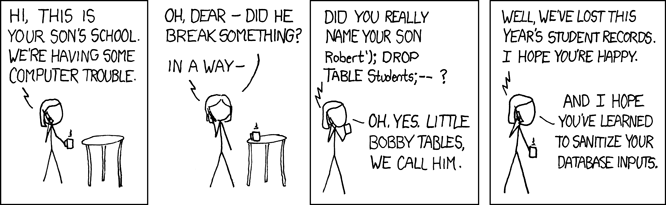
\includegraphics[scale=.5]{img/xkcd/exploits_of_a_mom.png}
\caption*{{\small \textit{Her daughter is named Help I'm trapped in a driver's license factory. (xkcd.com/327)}}}
\end{figure}
